\chapter{تحلیل و طراحی}

هدف از این فصل بررسی نیازمندی‌ها، تحلیل و طراحی معماری سامانه است. سامانه ذکر شده باید علاوه بر داشتن ویژگی‌های یک سیستم پایش شبکه، باید استفاده آن برای کاربر راحت و با کمترین دانش فنی قابل استفاده باشد. براي این که بتوانیم چنین سامانه‌اي را طراحی کنیم ابتدا باید نیازمندي‌هاي سامانه را تشخیص دهیم و سپس معماري کلی سامانه موردنظر خود را بر اساس فناوری‌های انتخابی به دست آوریم.
\\
در این فصل ابتدا نیازمندی‌ها تحلیل می‌شوند. بعد از آن فناوری‌های توسعه نرم‌افزار بررسی و انتخاب می‌شوند. و درنهایت معماری نرم‌افزار ترسیم می‌شود.



\section{تحلیل نیازمندی‌ها}

 بر اساس مطالعاتی که انجام شده و مطالب فصل قبل این سامانه باید ویژگی‌های زیر را داشته باشد:

\begin{itemize}
    \item کشف شبکه و ترسیم بصری آن برای ادراک بهتر توسط مدیر شبکه
    \item توانایی تنظیم پارامترهای مختلف عملکردی توسط مدیر شبکه از جمله دوره تناوب جمع‌آوری اطلاعات از عناصر
    \item جمع‌آوری اطلاعات مدیریتی و پردازش آن‌ها جهت تولید اطلاعات قابل فهم توسط مدیر شبکه
    \item ایجاد یک واسط کاربری مطلوب تحت وب و نمایش اطلاعات قابل فهم 
    \item فراهم آوردن حداقلی امنیت سیستم با استفاده از (\lr{SNMPv3} و پروتکل‌های دیگری که ایمن هستند)
    \item مقیاس پذیری سیستم جهت کارآمد بودن در هنگام افزایش وسعت شبکه
    \item فراهم آوردن یک بستری برای دریافت هشدارهای ارسالی عناصر تحت مدیریت
\end{itemize}

\newpage

به طور خلاصه هدف از انجام این پروژه توسعه یک ابزار پایش شبکه با ویژگی‌های پایه‌ای فوق است. به عبارتی هدف، افزودن یک امکان جدید به پروژه‌های موجود و پیاده‌سازی آن نیست، اما از زبان‌های برنامه نویسی و فناوری‌های بروز در مقایسه با پروژه متن باز زبیکس استفاده خواهد شد. به عبارت دیگر این پروژه از ابتدا بدون استفاده از کدهای متن باز موجود توسعه داده خواهد شد.



در ادامه نیز بعد از تحلیل نیازمندی‌های پروژه نیازمندی‌های کارکردی\LTRfootnote{\lr{functional requirements}} در جدول \ref{جدول نیازمندی‌های کارکردی} و غیرکارکردی\LTRfootnote{\lr{non functional requirements}} در جدول \ref{جدول نیازمندی‌های غیر کارکردی} آورده شده است.



\begin{table}[h!]
    \centering
    \caption{جدول نیازمندی‌های کارکردی}
    \label{جدول نیازمندی‌های کارکردی}
    \begin{tabular}{llp{5cm}} \toprule
        \multicolumn{1}{c}{ردیف} & \multicolumn{1}{c}{عنوان} & \multicolumn{1}{c}{شرح}  \\ \midrule
        \multicolumn{1}{c}1  & \multicolumn{1}{c}{کشف شبکه}  & {سامانه باید قادر باشد تا با دریافت یک آدرس شبکه، عناصری که عامل \lr{SNMP} بر روی آن‌ها فعال هستند را به همراه نوع عنصر(سرور، مسیریاب، سوئیچ و تکرارکننده) آن‌ها مشخص کند. این خروجی باید در قالب یک توپولوژی شبکه باشد.}   \\
        \multicolumn{1}{c}2  & \multicolumn{1}{c}{تنظیمات شبکه}  & {سامانه باید قادر باشد مشخصات عناصر مختلف از جمله نام کاربری، رمز عبور و ... را از کاربر دریافت کرده و مراحل بعدی طبق این مشخصات طی شوند. این مشخصات شامل پارامترهایی که کاربر جهت پایش مشخص می‌کند نیز می‌باشد.}   \\
        \multicolumn{1}{c}3  & \multicolumn{1}{c}{پردازش و ذخیره اطلاعات جمع‌آوری شده}  & {این سامانه باید بتواند اطلاعاتی که از شبکه جمع‌آوری می‌کند را پردازش و همچنین آن‌ها را در خود ذخیره کند.}   \\
        \multicolumn{1}{c}4  & \multicolumn{1}{c}{جمع‌آوری اطلاعات شبکه بر اساس تنظیمات شبکه}  & {این سامانه باید بتواند بر اساس تنظیماتی که کاربر بر شبکه اعمال کرده است، وضعیت هر عنصر تحت مدیریت را رصد و پایش کند.}   \\
        \multicolumn{1}{c}5  & \multicolumn{1}{c}{جمع‌آوری هشدارهای مربوط به عناصر تحت مدیریت}  & {این سامانه باید بتواند هشدارهایی که از سمت شبکه به سامانه وارد می‌شوند را به کاربر نمایش دهد.}   \\
    \end{tabular}
\end{table}

\newpage

\begin{table}[h!]
    \centering
    \caption{جدول نیازمندی‌های غیر کارکردی}
    \label{جدول نیازمندی‌های غیر کارکردی}
    \begin{tabular}{lp{8cm}} \toprule
        \multicolumn{1}{c}{عنوان} & \multicolumn{1}{c}{کیفیت} \\ \midrule
        \multicolumn{1}{c}{مدت زمان کشف شبکه}  & {شرح این کارکردی نیازمندی در جدول \ref{جدول نیازمندی‌های کارکردی} آمده است. این نیازمندی برای هر اجرا باید کمتر از دو دقیقه زمان ببرد.} \\
        \multicolumn{1}{c}{واسط کاربری مطلوب تحت وب}  & {این سامانه باید بتواند واسط کاربری تحت وبی ارائه کند، تا از راه دور در دسترس باشد. همچنین این واسط کاربری باید زیبا و کار با آن آسان باشد.} \\
        \multicolumn{1}{c}{امنیت سامانه برای جمع‌آوری اطلاعات}  & {این سامانه باید از آخرین نسخه \lr{SNMP} استفاده کند(\lr{SNMPv3}).} \\
        \multicolumn{1}{c}{امنیت سامانه برای ذخیره اطلاعات}  & {سامانه اطلاعاتی مهم از مشخصات عناصر مدیریتی در خود ذخیره می‌کند. باید مکانیزم‌های امنیتی برای ذخیره این اطلاعات اعمال شود. (استفاده از رمزهای عبور قوی برای پایگاه‌های داده و ...)} \\
    \end{tabular}
\end{table}
    
    





\section{بررسی و انتخاب فناوری پیاده‌سازی}

برای طراحی معماری سامانه ابتدا نیاز است تا فناوری‌های مورد استفاده معرفی شوند. به طور کلی نیز با توجه به نیازمندی‌ها، فناوری‌ها در چهار گروه واسط کاربری، سمت سرور\LTRfootnote{\lr{Back-end}}، هسته \lr{SNMP} و ذخیره‌سازی اطلاعات تقسیم می‌شوند. برای هر گروه در این بخش، ابتدا فناوری‌های موجود بررسی و درنهایت فناوری مورد استفاده نیز مشخص می‌شود.

\subsection{واسط کاربری}

برای توسعه واسط کاربری، هزینه توسعه پایین، زیبا بودن و راحتی کار با آن باید در نظر گرفته شود. البته ذکر این نکته نیز لازم است که واسط کاربری  باید تحت وب باشد تا از راه دور نیز قابل دسترس باشد. برای توسعه واسط کاربری با این مشخصات، چارچوب‌های\LTRfootnote{\lr{Frameworks}} ری‌اکت\LTRfootnote{\lr{React}}، انگولار\LTRfootnote{\lr{Angular}} و ویو جی‌اس\LTRfootnote{\lr{Vue.js}} مطرح هستند.

\newpage


\subsubsection{ری‌اکت}

یک کتابخانه متن باز توسعه یافته توسط فیسبوک است. این کتابخانه طبق نظرسنجی توسعه‌دهندگان استک اورفلو\LTRfootnote{\lr{Stack Overflow Developer Survey}} در سال 2021 م. توسط اکثر توسعه‌دهندگان واسط کاربری استفاده شده است. هدف اصلی این چارچوب رفع مشکلات نگهداری کد به دلیل استفاده مداوم کدها در برنامه است.


ری‌اکت به دلیل مدل شیء سند مجازی\LTRfootnote{\lr{Virtual Document Object Model (Virtual DOM)}}، عملکردی عالی از خود ارائه می‌دهد. همچنین برای کاربردهای با ترافیک بالا مناسب است. از طرفی به دلیل وجود مستندات کافی، برای توسعه‌دهندگان جدید یادگیری آن نسبتا راحت خواهد بود.



مزایا:
\begin{itemize}
    \item صرفه‌جویی در زمان در هنگام استفاده مجدد از اجزا
    \item یک چارچوب متن باز با ابزارهای متنوع
    \item مناسب برای برنامه‌های تک صفحه‌ای
    \item اکوسیستم بزرگ
\end{itemize}

معایب:

\begin{itemize}
    \item زمان یادگیری نسبتا طولانی
    \item چالش برانگیز بودن درک پیچیدگی های \lr{JSX}\LTRfootnote{\lr{JavaScript XML}} برای توسعه‌دهندگان
\end{itemize}

\newpage

\subsubsection{انگولار}

این چارچوب که بر اساس تایپ‌اسکریپت\LTRfootnote{\lr{Typescript}} است، به طور رسمی در سال 2016 م. منتشر شد. انگولار توسط گوگل ایجاد شد تا شکاف بین نیازهای روزافزون فناوری و مفاهیم  را کاهش دهد. برخلاف ری‌اکت، انگولار ویژگی اتصال داده\LTRfootnote{\lr{Two-way Data Binding}} را داراست. این بدین معنی است که یک همگام‌سازی زمانی بین نمایش\LTRfootnote{\lr{View}} و مدل وجود دارد. به عبارت دیگر هر تغییری در مدل به سرعت در نمایش و برعکس تکرار می‌شود. در مقایسه انگولار در مقابل ری‌اکت، یادگیری انگولار آسان نخواهد بود. با این حال، مستندات بی‌شماری در دسترس است.


مزایا:
\begin{itemize}
    \item فرایند آسان تولید کد
    \item اکوسیستم بزرگ
    \item عملکرد بالا
    \item سازگار با معماری‌های \lr{MVC}\LTRfootnote{\lr{Model–View–Controller}} و \lr{MVVM}\LTRfootnote{\lr{Model-View-ViewModel}}
\end{itemize}


معایب:

\begin{itemize}
    \item پیچیده بودن انگولار
    \item دشوار بودن جابجا کردن طرح‌های قدیمی از انگولار بر اساس جاوا اسکریپت به انگولار بر اساس تایپ‌اسکریپت
    \item زیاد بودن تلاش یادگیری
\end{itemize}


\newpage

\subsubsection{ویو جی‌اس}

یکی از ساده ترین چارچوب‌ها ویو جی‌اس است. با وجود اندازه کوچک آن دو مزیت اصلی دارد:

\begin{itemize}
    \item وجود مدل شی سند بصری
    \item مبتنی بر مؤلفه بودن آن 
\end{itemize}
همچنین از اتصال دو طرفه داده مانند انگولار بهره می‌برد.


تفاوت ویو جی‌اس و ری‌اکت در این است که ویو جی‌اس یک چارچوب جاوا اسکریپت\LTRfootnote{\lr{Javascript}} است در حالی که ری‌اکت یک کتابخانه جاوا اسکریپت است. بنابراین ویو جی‌اس برای پروژه‌های بزرگ مناسب‌تر است. اگرچه ویو جی‌اس برای مقابله با پیچیدگی‌ها و بهبود عملکرد برنامه ایجاد شده است، اما هنوز در میان صنعت‌های بزرگ محبوبیت زیادی ندارد. به طور مشابه، با مقایسه انگولار در مقابل ویو جی‌اس، ویو جی‌اس عملکرد انگولار را بهبود می‌بخشد.


مزایا:
\begin{itemize}
    \item مستندات کامل و دقیق
    \item سادگی و وضوح
    \item دارای ابزارهای توسعه دهنده مرورگر
    \item قابلیت استفاده مجدد کد و یکپارچه سازی ساده
\end{itemize}

معایب:

\begin{itemize}
    \item کوچک بودن جامعه توسعه‌دهندگان
    \item بی نظمی در کد به دلیل انعطاف پذیری 
\end{itemize}


\subsubsection{جمع‌بندی}

با توجه به موارد ذکر شده و زمان محدود برای پیاده‌سازی پروژه، کتابخانه ری‌اکت برای توسعه واسط کاربری استفاده شد. از جمله دلایل این انتخاب می‌توان به کوچک بودن جامعه توسعه‌دهندگان ویو جی‌اس و پیچیده بودن انگولار اشاره کرد. از طرفی نیازمندی‌های پروژه از امکاناتی که کتابخانه ری‌اکت در اختیار ما قرار می‌دهد، فراتر نخواهد رفت.


\subsection{سمت سرور}
برای توسعه سمت سرور و نوشتن \lr{APIs} بهترین گزینه‌های موجود فلسک\LTRfootnote{\lr{Flask}}، جنگو\LTRfootnote{\lr{Django}} و نودجی‌اس\LTRfootnote{\lr{Node.js}} بودند که در ادامه معرفی خواهند شد.

\subsubsection{فلسک}
فلسک یک چارچوب وب است که به زبان پایتون\LTRfootnote{\lr{Python}} نوشته شده است. ساختار فلسک واضح‌تر از چارچوب جنگو است و همچنین یادگیری آن آسان‌تر است زیرا کد کمتری برای پیاده‌سازی یک وب اپلیکیشن ساده نیاز دارد. فلسک از انعطاف بالایی برخوردار است. و همچنین از عملکردی ثابت در سراسر اجرای برنامه برخوردار است.

\subsubsection{جنگو }

جنگو نیز مانند فلسک یک چارچوب پایتون است که ساخت وب سایت با استفاده از پایتون را آسان‌تر می‌کند. جنگو از الگوی طراحی \lr{MVT}\LTRfootnote{\lr{Model View Template}} به صورت زیر پیروی می‌کند:

\begin{itemize}
    \item مدل: ارائه داده‌های مطلوب معمولا از پایگاه داده را برعهده دارد.
    \item نمایش: یک کنترل کننده درخواست که الگو و محتوای مربوطه را بر اساس درخواست کاربر برمی‌گرداند.
    \item الگو: یک فایل متنی حاوی طرح‌بندی صفحه وب، با منطق نحوه نمایش داده‌ها است.
\end{itemize}


\subsubsection{نودجی‌اس}
نودجی‌اس موتور جاوا اسکریپت وی هشت، هسته گوگل کروم را خارج از مرورگر اجرا می کند.

یک برنامه نودجی‌اس در یک فرآیند\LTRfootnote{\lr{Process}} واحد(بدون ایجاد یک ترد\LTRfootnote{\lr{Thread}} جدید برای هر درخواست) اجرا می‌شود. نودجی‌اس مجموعه‌ای از ورودی/خروجی‌های ابتدایی ناهمزمان را در کتابخانه استاندارد خود ارائه می‌دهد که از بلاک شدن کد جاوا اسکریپت جلوگیری می‌کند. این به نودجی‌اس اجازه می‌دهد تا هزاران اتصال همزمان را با یک سرور بدون وارد کردن بار مدیریت همزمانی رشته‌ها، که می‌تواند منبع مهمی از خرابی باشد، مدیریت کند.

\subsubsection{جمع‌بندی}
در قسمت توسعه سمت سرور فلسک انتخاب شد که دلایل آن را ادامه می‌بینید:
\begin{itemize}
    \item جنگو یک چارچوب برای توسعه همه‌جانبه\LTRfootnote{\lr{Full Stack}} یک سایت است که به دلیل آن که در این سامانه می‌خواهیم از \lr{APIs} استفاده کنیم جنگو مناسب این پروژه نخواهد بود.
    \item فلسک در مقایسه با نودجی‌اس کارایی کمتر و حتی سرعت پایین‌تری دارد، اما توجه به این نکته لازم است که سرعت این سامانه برای مدیریت درخواست‌های زیاد کاربردی برای ما نخواهد داشت؛ زیرا کاربران این سامانه محدود هستند.
    \item از طرفی به دلیل تولید داده بسیار توسط این سامانه، پایتون به دلیل وجود کتابخانه‌های متنوع و کارامد گزینه مناسب‌تری خواهد بود. 
\end{itemize}


\subsection{هسته \lr{SNMP}}
برای توسعه ابزاری برای مدیریت پیام‌های \lr{SNMP} به چندین زبان و کتابخانه می‌توان این کار را انجام داد. در ادامه برای سه زبان نکاتی که وجود دارد بیان می‌شود:

\begin{itemize}
    \item زبان \lr{C}: انتخاب به نسبت مناسبی خواهد بود. از این جهت که حتی ابزارهای نوشته شده برای لینوکس مانند \lr{snmpget} و ... با کتابخانه \lr{net-snmp} نوشته شده‌اند.
    \item زبان پایتون: برای توسعه این قسمت با زبان پایتون نیاز به استفاده از ماژول \lr{PySNMP} وجود دارد که به شدت کند است و با تعداد کمی از عناصر تحت مدیریت بر پردازنده سرور فشار زیادی وارد می‌کند.
    \item زبان ارلنگ\LTRfootnote{\lr{Erlang}}: زبان ارلنگ به صورت داخلی از \lr{SNMP} پشتیبانی می‌کند. و در آزمایشاتی حتی از زبان‌های \lr{C} یا \lr{C++} بهتر عمل کرده است. اما با توجه به محدودیت زمانی توسعه پروژه و همچنین نا آشنا بودن با زبان ارلنگ این زبان تست نشد.
\end{itemize}

و درنهایت از زبان \lr{C} و کتابخانه \lr{net-snmp} برای توسعه انتخاب شد.


\subsection{ذخیره‌سازی اطلاعات}

در پیاده‌سازی این سامانه اطلاعاتی که باید ذخیره شوند به شرح زیر می‌باشد:
\begin{itemize}
    \item هشدارهای دریافتی از سمت عناصر تحت مدیریت
    \item اطلاعات جمع‌آوری شده برای برای یک پارامتر خاص از عناصر تحت مدیریت
    \item اطلاعات کاربرانی که توسط یک ادمین ارشد تعریف می‌شوند
    \item اطلاعات شبکه‌(توپولوژی، عناصر تحت مدیریت و ...)

\end{itemize}

داده‌های مربوط به دو مورد اول به صورت خیلی سریع تولید می‌شوند. همچنین نیاز به بازیابی سریع و مداوم آن‌ها نیز موجود دارد. اما از طرفی داده‌های مربوط به دو مورد آخر هم دارای ساختار هستند و هم مقدار دسترسی به این نوع داده‌ها زیاد نیست. با توجه به موارد ذکر شده برای دو مورد اول به دلیل داده زیاد و سرعت بازیابی بهتر از پایگاه‌داده‌های در حافظه اصلی\LTRfootnote{\lr{In-Memory Database}} استفاده می‌کنیم. همچنین برای دو مورد بعدی از پایگاه‌داده‌های رابطه‌ای\LTRfootnote{\lr{Relational Databases}} مناسب هستند.
\\
برای انتخاب پایگاه‌داده‌ در حافظه اصلی یکی از بهترین گزینه‌ها ردیس\LTRfootnote{\lr{Redis}} خواهد بود. ردیس به دلیل رایگان بودن، سرعت بازیابی بالا ، پایین بودن حجم داده ذخیره شده و ... نسبت به رقبا برتری محسوسی دارد.
\\
برای انتخاب پایگاه‌داده رابطه‌ای نیز با توجه به چارچوب انتخابی سمت سرور(فلسک(پایتون)) \lr{ SQLite} بهترین انتخاب خواهد بود. به طور کلی از سازگارترین پایگاه‌های داده با فلسک میتوان به \lr{SQLite} و \lr{ MySQL} اشاره کرد. از طرفی برای کار با \lr{ SQLite} نیاز به نصب هیچ بسته نرم‌افزاری برای کار با آن نیست و در پایتون تعبیه شده است.



\newpage

\section{معماری سامانه}




با توجه به مطالبی که در این فصل تا به اینجا گفته شد، سامانه پایش شبکه‌های کامپیوتری به ماژول‌های زیر تقسیم می‌شود \cref{fig.11}. ابتدا یک ماژول تحت عنوان هسته \lr{SNMP} در نظر گرفته می‌شود که وظیفه مدیریت پیام‌ها و پیاده‌سازی پروتکل به یک زبان برنامه نویسی خاص است.




\begin{figure}[!h]
\centering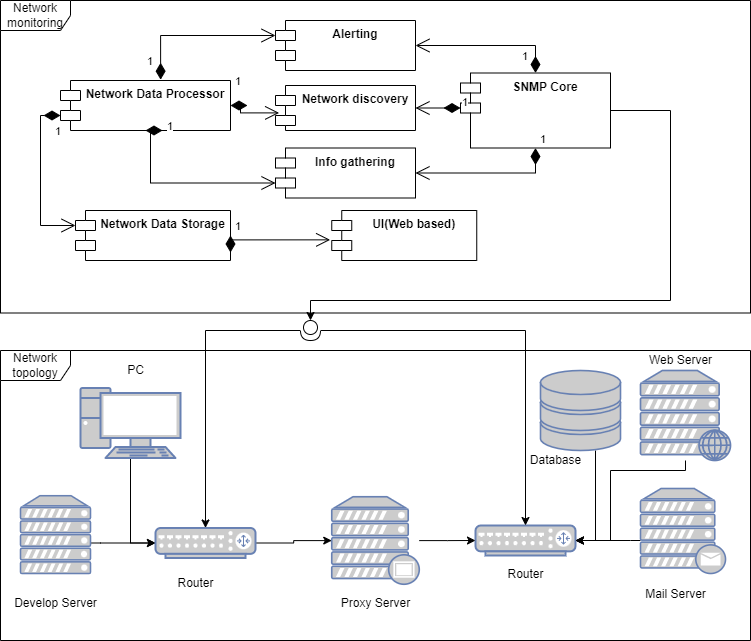
\includegraphics[scale=.55]{./diagram}
\caption{نمودار بلوکی اجزای سامانه}\label{fig.11}
\end{figure}


سپس ماژول کشف عناصر تحت مدیریت شبکه در نظر گرفته می‌شود، که به کمک ماژول هسته وظیفه جمع‌آوری اطلاعات ساختاری شبکه را بر عهده دارد. بعد از آن ماژول جمع‌آوری اطلاعات، عملکرد کل شبکه را رصد می‌کند. حال اگر زمانی با توجه به وجود اعلان‌ها نیاز به هشدار وجود داشت، از ماژول هشدار استفاده می‌شود. 

\newpage

نکته حائز اهمیت در رابطه با سه ماژول آخر این است که هر ماژول از ماژول هسته استفاده می‌کند. همچنین اطلاعاتی که هر ماژول بدست می‌آورد تحویل ماژول پردازش اطلاعات می‌دهد.

در پردازشگر اطلاعات شبکه، اطلاعات خام دریافتی از سه ماژول هشدار، کشف شبکه و جمع‌آوری اطلاعات پردازش می‌شوند تا اطلاعات قابل فهم توسط مدیر استخراج شود. حال باید اطلاعات تولید شده به ماژول ذخیره‌سازی اطلاعات داده شود.

ماژول واسط کاربری نیز در قالب یک وب سایت و فراهم آوردن یک پنل ورودی برای مدیران شبکه نیز اطلاعات ساختاری شبکه، پایش شبکه و هشدارها را از ماژول ذخیره‌سازی دریافت کرده و نمایش می‌دهد. همچنین از طریق آن می‌توان پارامترهای مختلف برای عناصر مختلف تنظیم و اقدام به اسکن کل شبکه کرد.

اما نیاز است که یک واسطی بین شبکه و سامانه مذکور باشد. در شکلی که بررسی شد، سامانه به یک شبکه فرضی از طریق مسیریاب‌های آن متصل است. در واقع واسط بین سامانه و شبکه ماژول هسته \lr{SNMP} خواهد بود.






\section{خلاصه}
% 1


هدف نهایی این فصل طراحی معماری سامانه بود. برای این امر ابتدا زیرمجموعه‌ای از ویژگی‌های سامانه‌های فصل دوم ذکر شد.

سپس با تحلیل نیازمندی‌ها دو جدول نیازمندی‌های کارکردی و غیرکارکردی تولید شد. در نهایت بعد از تولید نیازمندی‌ها به بررسی فناوری‌های پیاده‌سازی بخش‌های مختلف پرداخته شد. در نهایت نیز با توجه به فناوری‌های انتخاب شده، معماری جهت توسعه نرم‌افزار طراحی شد.

